\documentclass{TISE}

% additional packages
\usepackage{etoolbox}
\usepackage{float}
\usepackage{soul}
%\AtBeginEnvironment{quote}{\small}

% title info
\title{Not just normal: exploring power with Shiny apps}
\author{Christian Stratton and Dr. Jennifer L. Green \\ Montana State University}

\begin{document}
	
\section{INTRODUCTION}

Statistical power is a fundamental component of most graduate and undergraduate mathematical statistics courses, and yet it is frequently cited as one of the most difficult topics to teach \citep{aberson2002}. This difficulty is driven by the conceptual richness of the topic. To fully understand power, students must understand the relationship between the sampling distributions of the test statistic under both the null and alternative parameter spaces and how they are used to compute power, as well as the factors that influence those distributions. Guiding students towards a conceptual understanding of these relationships can be challenging, as the relationships are difficult to visualize using traditional classroom methods \citep{aberson2002}.

In traditional upper-level mathematical statistics courses, such as curricula based on \cite{wackerly2008} or \cite{casella2002}, exploration of power is typically done through the definition of power and derivations of power functions. \cite{casella2002} define power by considering a hypothesis test of $H_0 : \theta \in \Theta_0$ versus $H_1 : \theta \in \Theta_0^c$ and defining $\mathcal{R}$ as the rejection region for that test. They then define the power function of this test as $\beta(\theta) = P(\boldsymbol{X} \in \mathcal{R} | \theta)$. In words, the power function represents the probability of rejecting the null hypothesis for a given value of $\theta$. \cite{casella2002} follow this definition with derivations of the power function for samples from the binomial and normal population distributions, respectively. This method of presenting and exploring statistical power - largely through computational mechanics - is mirrored in many of the traditional curricula based on this text. 

From the definition and derivation of a hypothesis test's power function, students are expected to understand a range of learning objectives. Potential learning objectives for power include but are not limited to:
\begin{itemize}
	\item[1)] understanding how the sample size, null value, alternative hypothesis, significance level, the test statistic, and the population distribution each affect power;
	\item[2)] understanding the relationship between the power function and the sampling distribution of the test statistic under both the null hypothesis and true value of $\theta$; and
	\item[3)] understanding how to calculate the power of a hypothesis test using a variety of strategies.
\end{itemize}

However, students' conceptual understanding of complex topics such as power can be greatly enhanced by the use of graphical and visualization techniques (\cite{chance2007}; \cite{delMas1999}; and \cite{bobek2016}). The \textit{Guidelines for Assessment and Instruction in Statistics Education} (GAISE) for introductory statistics at the college level has also promoted using technology to provide students with visual representations of complex topics \citep{ASA2005}. The American Statistical Association recently extended these expectations to undergraduate degree programs. The \textit{2014 Curriculum Guidelines for Undergraduate Programs in Statistical Science} \citep{ASA2014} places renewed vigor on developing undergraduate statistics curriculum that allow students to develop a conceptual understanding of the material and think critically. \cite{green2015} describe various tools that can be used to foster active learning and conceptual understanding of the concepts discussed in a traditional mathematical statistics curriculum; among these tools is the use of technology and visualizations.

To create visualizations that allows students to develop a conceptual understanding of power, students must first derive multiple power functions - for differing population distributions, statistics, and alternative hypotheses - and then plot the functions using statistical software. While there is value to each of these steps, the time commitment and difficulty of the task may frustrate students and distract from understanding the learning objectives. Alternatively, instructors may create graphics either during class in real-time or in advance. The former case requires substantial coding experience on the part of the instructor and demands class time, and the latter case can be restrictive in that it does not allow the students an organic exploration of the factors that affect the power function as the visuals were created by the instructor in advance.

To resolve this issue, instructors may used web-based applications when teaching power that allow students to make interactive discoveries using point-and-click graphical interfaces. Use of such applications allows students access to graphical representations of power without the need for either the student or the instructor to develop those visualizations. There already exist many exceptional graphical tools for understanding statistical power (\cite{aberson2002}; \cite{andersoncook2003}; and \cite{rossman2004}), though many assume samples are drawn from a normal population and were created for introductory courses. As noted by \cite{doi2016}, it can be difficult to find an existing application that perfectly suits the needs of an instructor. In such a case, instructors may either adapt a currently existing application, which requires access to source code and literacy in the source coding language, or develop one of their own, which requires a significant time investment and knowledge of many different coding languages. 

We desired a web application that allowed students to explore what factors affect the power function for many different test statistics assuming population distributions beyond the normal distribution. Additionally, we wanted students to be able to visualize both the power function and the sampling distributions of the test statistic over the null and alternative parameters spaces by interacting with the power function. These goals motivated the development of our web application. The rest of this article is laid out as follows: in Section 2, we discuss how the layout and features of the application are designed to help promote students' conceptual understanding of power through the use of visualizations; in Section 3, we describe how this web application can be used to address the learning objectives provided above; in Section 4, we discuss our experience implementing this web application and provide student reflections; in Section 5, we conclude with a discussion of the value of this web application and opportunities for future work. 

\section{APPLICATION LAYOUT}

When designing this web application, we had two primary goals. First, we wanted to develop a tool that allows students to visualize the relationship between the power function and various factors that influence it. In particular, we wanted students to be able to explore the effect of the population distribution, statistic of interest, null value, alternative hypothesis, significance level, and sample size on the power function in real time without needing to derive or plot that function. We also wanted to allow students to visualize the relationship between the power function and the sampling distribution under both the null hypothesis and true value of theta in order to develop a conceptual understanding of how power is derived. The development of such a web tool provides an efficient way to support students' conceptual understanding of power and sampling distributions through visualizations without spending class time creating them. These goals led to the development of the {\sf R} Shiny application provided in Figure 1. 

This web application features three different families of population distributions: the exponential($\theta$) family, the normal($\theta$, $\sigma^2$) family, and the uniform(0, $\theta$) family of distributions. For any population distribution, three statistics are available: the sum of the random variables, the sample minimum, and the sample maximum. For each combination of population distribution and statistic, there are three alternative hypotheses available: a not equal to alternative, a greater than alternative, and a less than alternative. And finally, the user has the option to specify the sample size, significance level, and null value. Based on these options, the power curve is plotted in the main plotting window. Beneath that, the sampling distribution of the statistic under both the null hypothesis and true value of $\theta$ is plotted once the respective point on the power curve is clicked. 

We chose to create this application in {\sf R} Shiny because of its use of reactive programming. Reactive programming allows the application to tailor output based on user input in real time. This is particularly useful when exploring power as it allows users to investigate the relationship between the power curve and sampling distribution of the statistic in an interactive way. In this web application, the user is able to visualize the sampling distribution of the statistic for a particular value of $\theta$ by either clicking on a point on the graph of the power function or by specifying the value in the ``Theta" box on the side panel (\hl{Figure 2}). Note that this plot is not visible until $\theta$ is specified using one of these two options. Additionally, both plots respond in real-time to any changes in the options provided on the side panel. This allows users of the application to quickly assess the impact of any of those changes on both the power function and the sampling distributions, thereby helping them understand the relationship between the options on the sidebar, the power function, and the sampling distributions. 

\newpage

\begin{figure}[H]
	\centering
	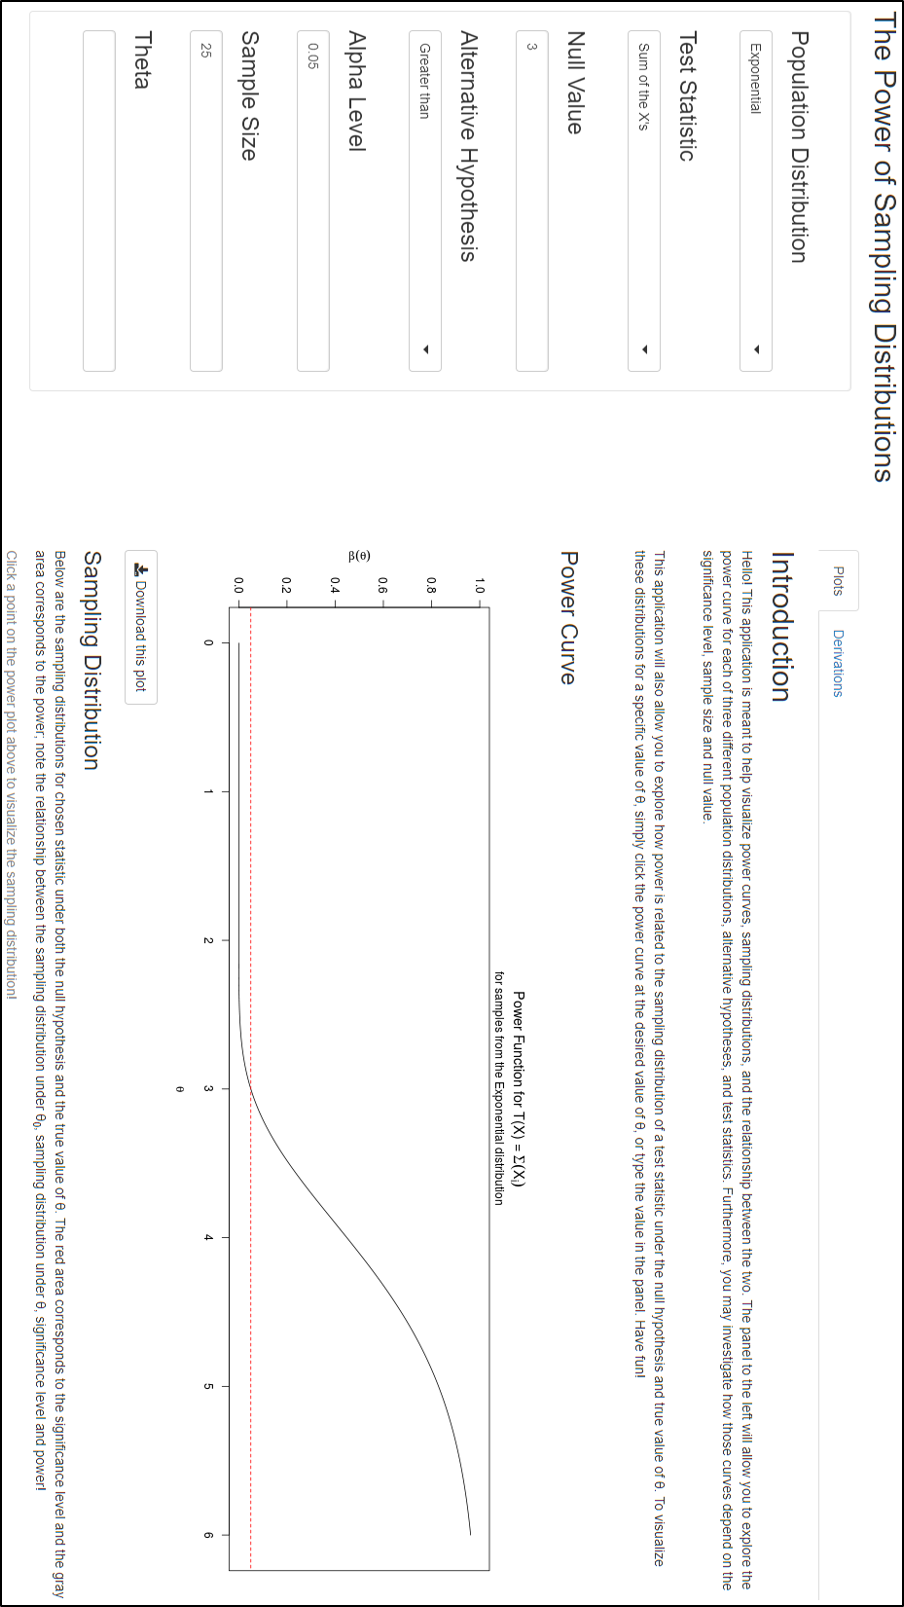
\includegraphics[scale=1]{app_layout.png}
	\caption{Interface for this web application. In the side panel, users may specify the population distribution, test statistics, null value, alternative hypothesis, significance level, and sample size. Based on these selections, the power curve is created in the main plotting window in real-time.}
\end{figure}

\newpage

\begin{figure}[H]
	\centering
	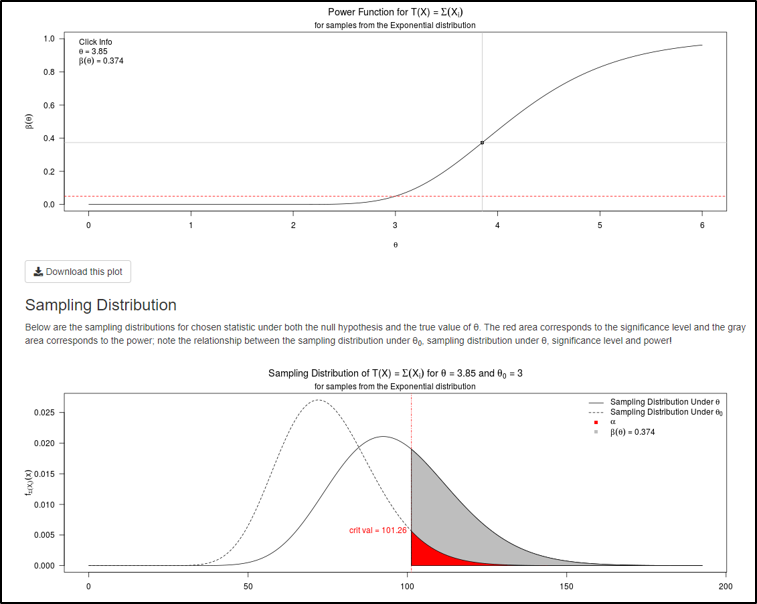
\includegraphics[scale=1]{reactive.png}
	\caption{Power function for a hypothesis based on the sum of random variables for a sample of size 25 from the exponential distribution assuming a greater than alternative hypothesis, significance level of 0.05, and null value of 3. The sampling distribution plot is created once a point on the power curve is selected and updated in real-time based on any subsequent changes to inputs on the side panel or theta.}
\end{figure}

We compartmentalized many of the features of this application to allow users to focus on specific topics rather than other potentially distracting features. For example, the conditionality of the sampling distribution plot allows users to explore relationships between the options on the sidebar and the power function before considering sampling distributions. In addition, this web application presents distribution specific options. For example, specification of the population standard deviation, $\sigma$, is only available when the normal distribution is selected. A host of other options appear when both the uniform distribution and sum of random variables are selected, allowing the user to explore the numerical instability present in the distribution function associated with that statistic when sampling from the uniform distribution (see Section 3.3 for discussion). By consciously hiding certain options and tabs when they are not needed, the user is able to focus on learning without added distractions. 

In addition to these structural features, we included features to make the application more user friendly, including  download options for each of the created plots and tabs to work through the derivations of each power curve. The download option allows for easy sharing and collaborative explorations within a classroom. In our experience, students were asked to investigate a particular relationship (e.g., the relationship between sample size and the power function) and upload images supporting their findings to a shared Google document which was then used for class discussion. If desired, the derivations tab allows users to work through the derivations for each of the power functions provided in the plots tab (\hl{Figure 3}). Although the focus of this application is on developing understanding through visualizations, we included the derivations to help users build connections between the graphical and mathematical representations of power.

\begin{figure}[H]
	\centering
	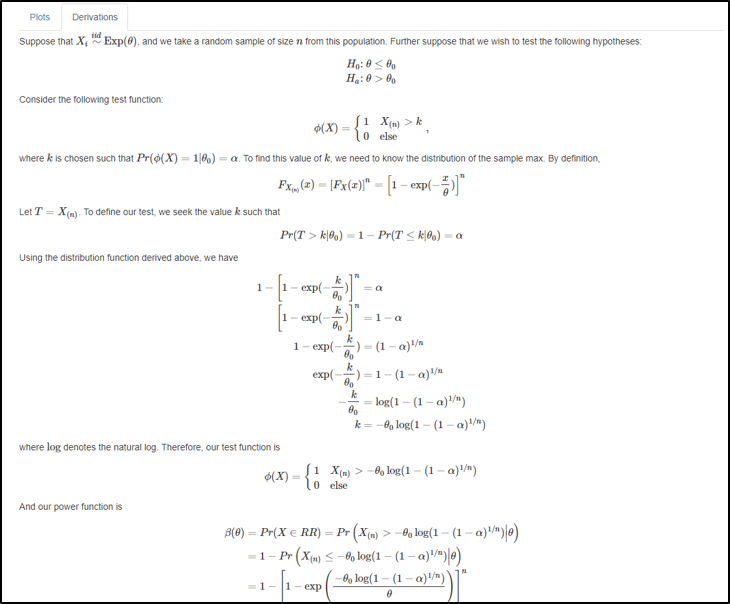
\includegraphics[scale=1]{derivs.png}
	\caption{Power function derivations for a hypothesis test based on the sample maximum for samples drawn from an exponential population assuming a greater than alternative hypothesis. The population distribution, test statistic, and alternative hypothesis are selected using a sidebar panel (not pictured).}
\end{figure}

This web application was consciously designed to support students' learning of power through the reactive nature of Shiny, our choice to compartmentalize application features, and several user friendly additional features. In the next section, we discuss how this conscious design can be used to address each of the learning objectives provided in Section 1.

\section{APPLICATION EXPLORATIONS}

An advantage of teaching power through this web application is that it allows for creativity and flexibility in how the instructor approaches the topic. Through tabular panels and conditional plots, this applet can aid instructors in accentuating a number of different fundamental aspects of power, yet also allow students to explore at their own pace. In this section, we describe how this applet may be used to explore the learning objectives defined in Section 1. Section 3.1 focuses on power curves and how they change for different population distributions, test statistics, null values, alternative hypotheses, alpha levels, and sample sizes; Section 3.2 focuses on how those curves arise by examining sampling distributions of test statistics under a number of different conditions; and finally, the Section 3.3 explores alternatives to traditional methods of determining power.

\subsection{Exploring power curves}

Statistical power is a complex concept that is influenced by several factors, including the distribution from which one is sampling, the statistic chosen to summarize the sample, the hypothesis of interest, the significance level, and the number of observations drawn from the population. As noted in Section 1, these relationships are often examined through the derivation of a power curve, but students' conceptual understanding of these relationships can be greatly enhanced through the use of visualizations. Creating these visualizations requires fluency in a coding language and mathematical expertise, as well as devotion of class time towards creating them. 

The use of this web application can help alleviate these requirements by allowing students to visualize relationships between the power curve and a host of different factors without having to derive the power function and code required to plot that function. For the remainder of this section, we explore each of the factors that affect the power curve and highlight how this applet may be used to make connections between the power curve and each of those factors.

\subsubsection{Varying the population distribution}

The role of the population distribution in a power function is one of the more abstract relationships we consider in this application, as it only manifests through the functional form of the power function. Consequently, it can be a difficult topic to explore without visuals. This web application provides an easy way to explore this relationship as it allows the user to quickly switch between population distributions while holding the statistic, null value, alternative hypothesis, significance level, and sample size constant. Students can be guided through this exploration by asking them to fix a particular combination of these factors while varying the population distribution of interest. \hl{Figure 4} provides such a suite of plots for a hypothesis test based on the sample maximum with a greater than alternative hypothesis, a null value of 3, a significance level of 0.05, and a sample size of 25.

\hl{Figure 4} guides students towards discussing how quickly each of the power functions are increasing as $\theta$ increases. Students must understand what $\theta$ represents in each of these populations, as well as what a power function represents at each value of $\theta$, which is a fundamental learning objective when considering power. Students may also be prompted to discuss which power function is closest to an ideal power curve. To answer such a question, students must first consider what an ideal power function looks like for the alternative hypothesis of interest, which further reinforces their understanding of what a power function represents at each value of $\theta$. Addressing this question also entails considering the behavior of the power function over both the null and alternative parameter spaces, and how that behavior relates to the alternative hypothesis. Following these questions, students may be asked to brainstorm what other factors might affect the power function, each of which may be explored by varying other options on the web application.

\begin{figure}[H]
	\centering
	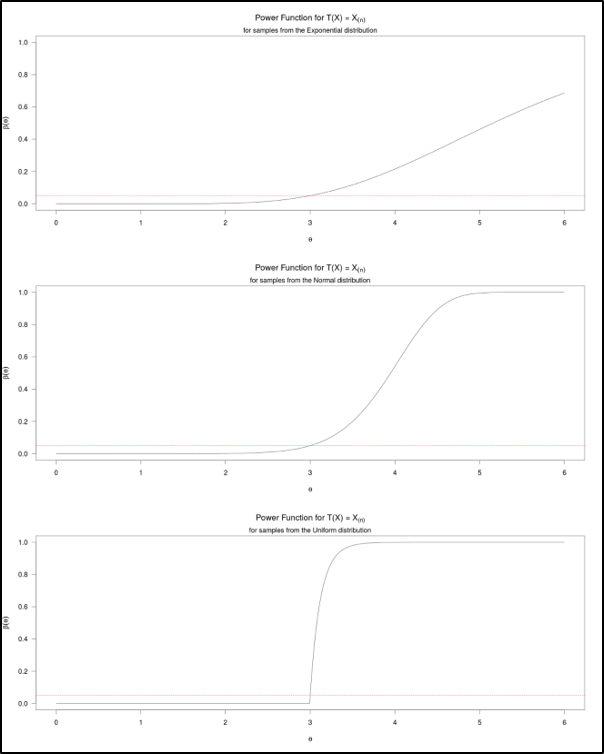
\includegraphics[width=4in]{varypop.png}
	\caption{Comparison of the power function for the sample maximum from each of the exponential (top), normal (middle), and uniform (bottom) distributions.}
\end{figure}

\subsubsection{Varying the test statistic}

In standard mathematical statistics courses (e.g., \cite{casella2002}), students are often asked to use power curves to compare test functions based on different test statistics. Students can make such comparisons by providing a specific combination of factors in the side panel of this web application. For example, \hl{Figure 5} provides a set of plots comparing each of the available statistics for the uniform and normal population distributions (assuming a null value of 3, significance level of 0.05, not equal to alternative hypothesis, and sample size of 25).

From \hl{Figure 5}, students may be asked to identify which power function is closest to ideal for each population distribution. This question helps students understand that the test statistic that provides the highest power in the alternative space depends upon the population distribution of interest. By choosing this particular combination of statistics and population distributions, students may be asked to think critically about why the sum of random variables performs best for the normal distribution and why the sample maximum performs best for the uniform distribution. This avenue of exploration can lead to discussions of sufficiency in the context of power thereby helping students draw connections between power and previously explored topics.  

\begin{figure}[H]
	\centering
	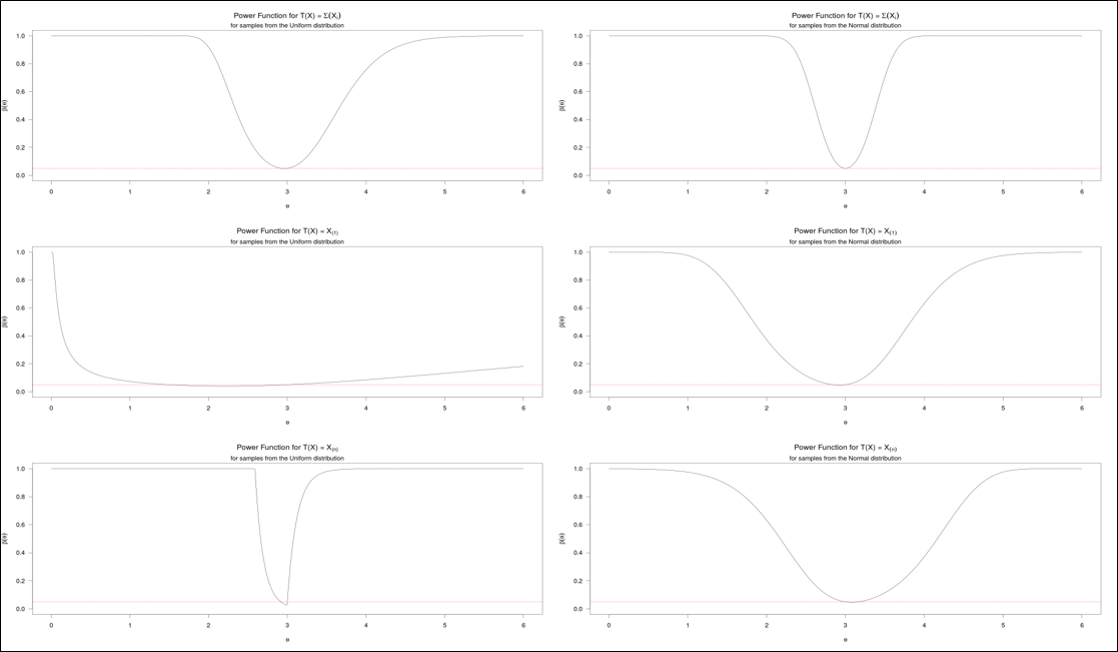
\includegraphics[width=\textwidth]{varystat.png}
	\caption{Comparison of power functions for varying statistics and population distributions. The left and right columns correspond to samples from the uniform and normal distribution, respectively. The top, middle, and bottom rows correspond to test functions based on the sum of random variables, sample minimum, and sample maximum, respectively.}
\end{figure}

\subsubsection{Varying the alternative hypothesis}

This web application can also be used to help students understand the effect of the alternative hypothesis on the power curve. Varying the alternative hypothesis while holding all other aspects of the power curve constant allows students to consider the relationship between the null and alternative parameter spaces and what the power function represents across each of these spaces. For example, \hl{Figure 6} showcases this exercise for a hypothesis test based on the sum of variables for samples of size 25 from the exponential distribution. 

From \hl{Figure 6}, students may easily visualize the effect of the alternative hypothesis on a power function; namely that for well-behaved tests, we expect greater power over the alternative parameter space than over the null parameter space. 

\begin{figure}[H]
	\centering
	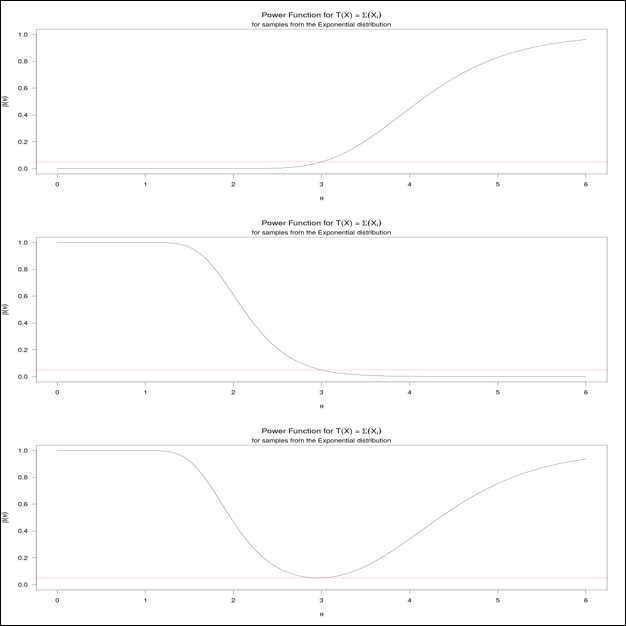
\includegraphics[scale=1]{varyalt1.png}
	\caption{Comparison of alternative hypotheses for hypothesis tests based on the sum of random variables when sampling from the exponential distribution. The top row corresponds to a greater than alternative, while the middle and bottom represent a less than and not equal to alternative, respectively.}
\end{figure}

Students can also be asked to consider bias in a testing context by guiding them to look at the power function for the sample maximum from the uniform distribution (\hl{Figure 7}). This power function provides an example of an unbiased test, which is rarely explored in a traditional power curriculum.

\newpage

\begin{figure}[H]
	\centering
	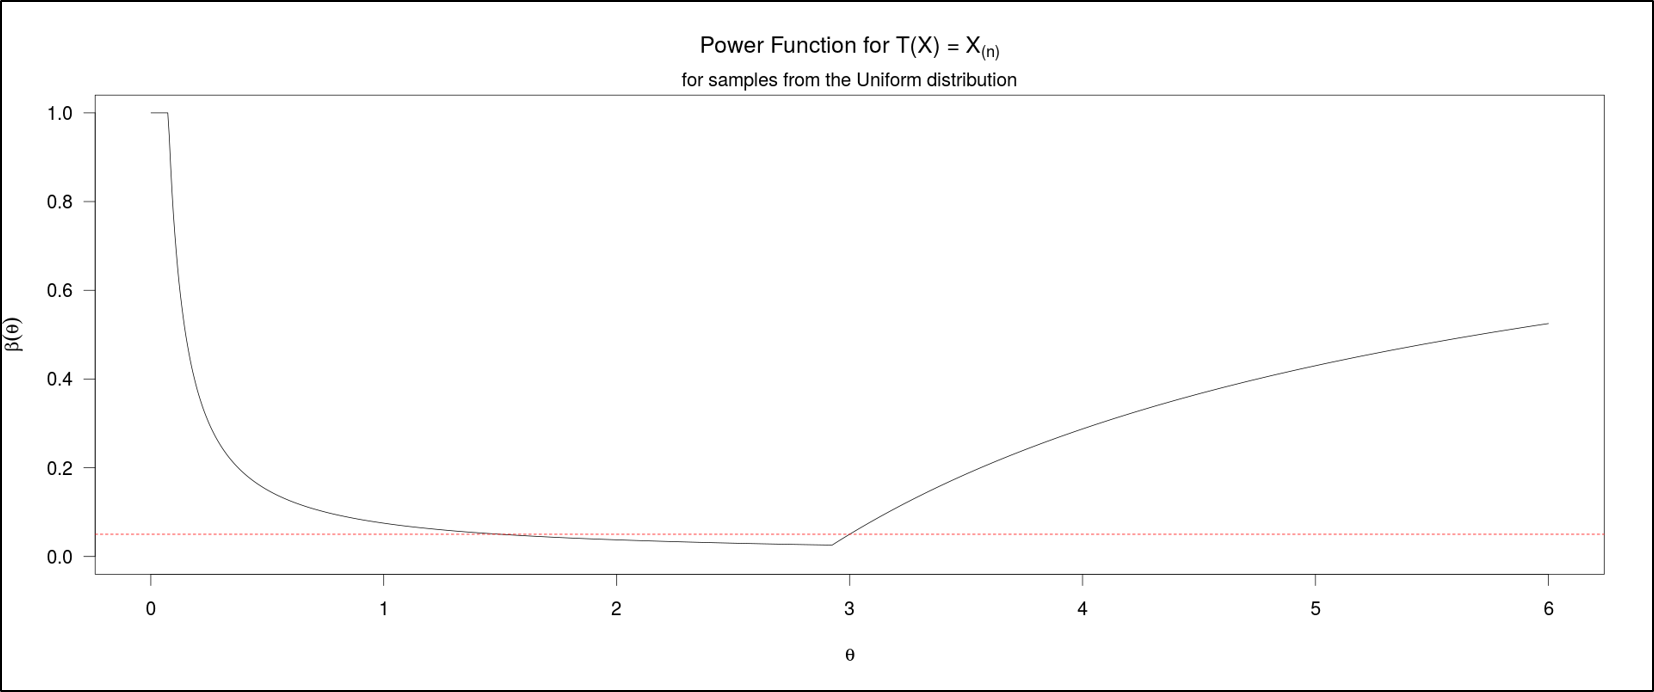
\includegraphics[width=\linewidth]{varyalt2.png}
	\caption{Power function for a hypothesis test based on the sample maximum assuming a sample of size one is taken from the uniform distribution.}
\end{figure}

This example is particularly interesting as the test is based on a complete, sufficient statistic and yet is biased. This apparent dichotomy motivates students to consider the advantages and disadvantages that may come with choosing certain statistics in different testing situations, offering rich classroom discussions. 

\subsubsection{Varying the significance level and null value}

The significance level plays a key role in determining power as it is used to determine the critical values of a hypothesis test and also represents the type I error rate. To help students understand how the significance level and null value are used to define a hypothesis test, students may be asked to vary the significance level and null value while leaving the other factors on the sidebar of the web application constant. \hl{Figure 8} depicts this exercise from an exponential population. 

From \hl{Figure 8}, students are able to visually determine that for size $\alpha$ tests, the power of the test at the null value is equal to the significance level. They are also able to see that larger significance levels lead to greater power over both the null and alternative parameter spaces. Building this conceptual understanding of the effect of the significance level and null value on the power function may help students better understand how to derive a test function. 

In addition to this mechanical effect of the significance level and null value on the power function, students can be pushed to consider more abstract relationships, such as the relationship between the power of a test and the type I error rate. Since the significance level is the type I error rate for size $\alpha$ tests, a compromise must be made between increasing the power of the test across the alternative space and increasing the type I error rate when determining the appropriate significance level for a test. This compromise is easy to visualize from \hl{Figure 8}, which provides an opportunity to discuss the responsibility of the researcher in hypothesis testing in the classroom setting.

\begin{figure}[H]
	\centering
	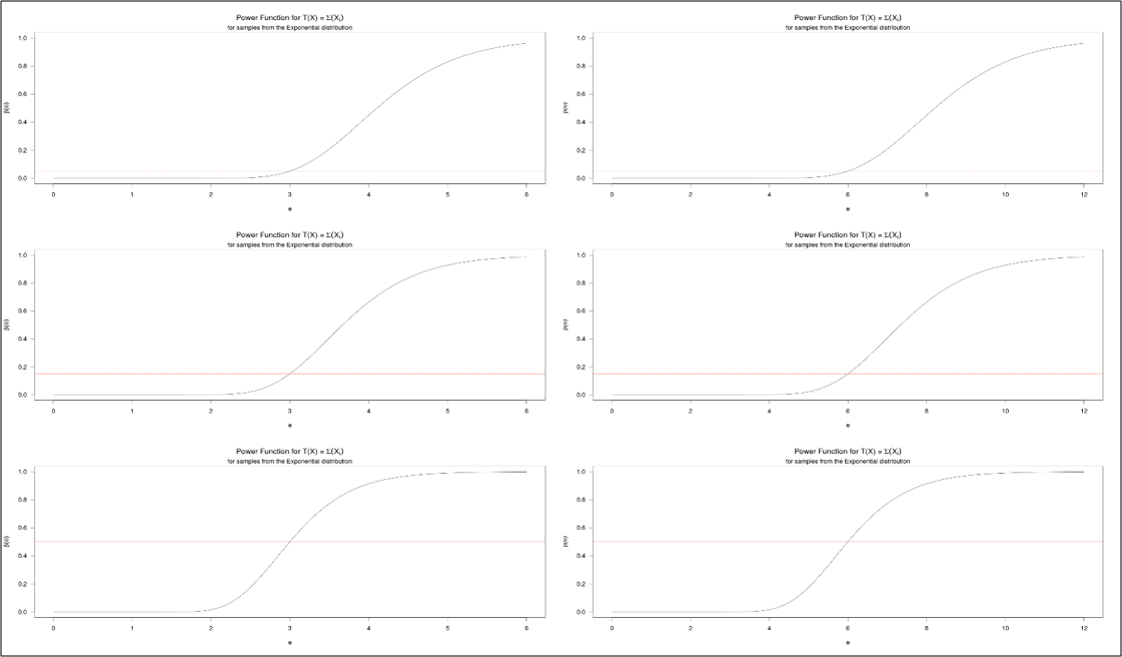
\includegraphics[width=\linewidth]{varyingsig.png}
	\caption{Comparison of power functions for varying significance levels and null values. The left and right columns correspond to null values of three and six, respectively. The top, middle, and bottom rows correspond to significance levels of 0.05, 0.15, and 0.5 respectively.}
\end{figure}

\subsubsection{Varying the sample size}

The last factor we consider is the sample size, which is often of interest when conducting power analyses. In general, as the sample size increases, so too does the power over the alternative parameter space. To help students understand this relationship, they may be asked to vary the sample size while holding all other factors constant. As an interesting example, \hl{figure 9} depicts this exercise for both the sum of random variables and sample minimum from the normal distribution. 

From this figure, students may easily determine the effect of the sample size on the power function. It also provides an opportunity to discuss why the sample size has a greater effect on the power function for the sum of random variables than it does on the power function for the sample minimum. Such a discussion requires students to consider why it is easier to determine that $\theta$ differs from the null value when considering a sum of normal random variables than when considering the sample minimum for a given sample size. In doing so, students must consider the sampling distribution of each statistic, which can be further explored in the next section.

\newpage

\begin{figure}[H]
	\centering
	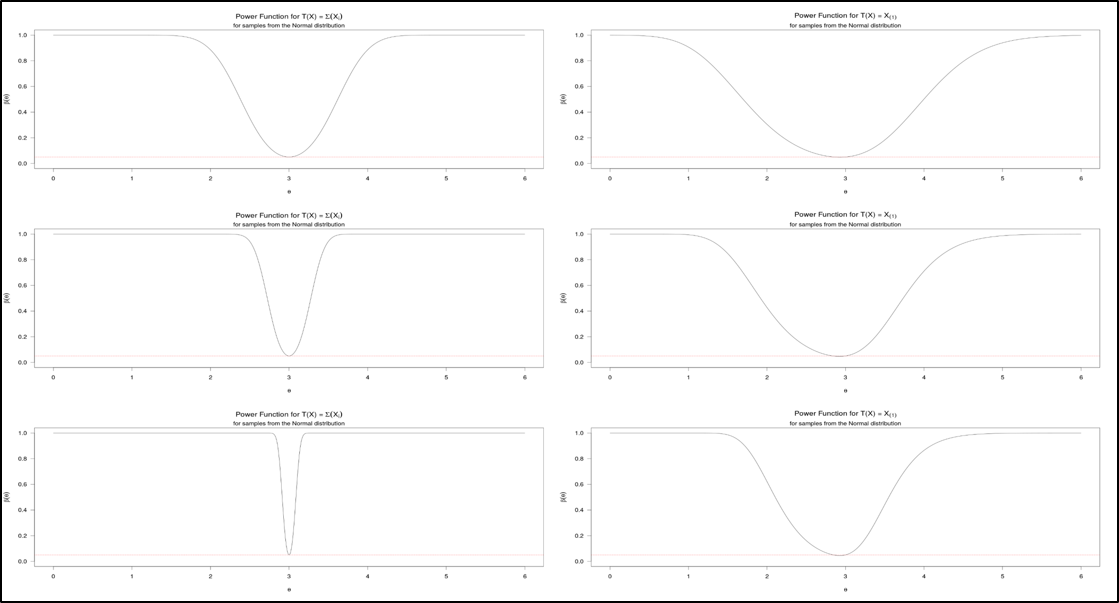
\includegraphics[width=\textwidth]{varyingn.png}
	\caption{Comparison of power functions for varying statistics and sample sizes for samples from the normal distribution. The left and right columns correspond to the sum of the random variables and the sample minimum, respectively. The top row corresponds to a sample size of 10, the middle row to a sample size 50, and the last row to a sample size of 500.}
\end{figure}

\subsection{Exploring sampling distributions}

One of the more conceptually challenging aspects of learning power is understanding why the power function is a function of theta and how that function relates to the sampling distribution of the statistic under the null hypothesis. This relationship is often explored graphically, though doing so requires both deriving the sampling distribution of a statistic and plotting that sampling distribution with statistical software. This web application allows the user to view the sampling distribution of the chosen statistic under the null hypothesized value of theta and a user specified value of theta for many different statistics and population distributions without having to work through any derivations. 

With this web application, students may click multiple points along the power curve and describe the resulting plot under the sampling distribution heading. Through this process, students recognize that there is an implied sampling distribution of the statistic under both the null hypothesis and true value of theta for each point along the power curve (\hl{Figure 2}). Since these plots update in real-time, students can click many points along the power curve to see how the sampling distribution of the statistic changes as the power changes. Through this process they are also able to visualize how the sampling distribution under the null hypothesis is static and does not depend on the chosen value of theta. This exploration is valuable as it makes the dependence of the power function on theta graphically explicit.

Once students have explored the sampling distributions for the statistic under the null hypothesis and true value of theta, the next key learning objective is to understand how power is determined from those distributions. In \hl{Figure 2}, the power is represented by the larger gray area and the significance level is represented by the smaller red area. From this graphic, students can visually assess how the significance level is used to determine the critical value, which is in turn used to calculate the power. Developing this conceptual understanding of how power is determined may help inform the derivation process for students and develop an intuition for how one might simulated power, which is further discussed in section 3.3.

Exploring what factors affect power functions and how that function relates to the sampling distribution of the statistic under both the null hypothesis and true value of $\theta$ fulfill the first two learning objectives provided in section 1.1. In the next section, we investigate the final learning objective by describing how this web application can be used to explore alternative methods of determining power, such as through normal approximations via the Central Limit Theorem or through simulation.

\subsection{Exploring other methods}

In the previous sections, we have largely focused on combinations of population distributions and statistics for which the distribution of the statistic is known in closed form and the power function is therefore readily obtainable. However this is not always the case when investigating power. In some cases, issues may arise that make it difficult to derive the formula for or visualize the power function. Learning how to resolve the issues that arise in these cases is valuable for students as it not only prepares them for potential challenges that they may encounter as a practicing statistician but also improves their ability to think critically and reason quantitatively. 

One issue a practicing statistician may encounter is that of numerical instability in the distribution function of the statistic of interest. For even modest sample sizes, the sampling distribution of the sum of uniform($0, \theta$) random variables exhibits numerical instability that manifests in the form of a strange oscillating pattern in the sampling distribution which is visible in the power function (see \cite{alberto2019} for more detail); this instability is exacerbated for larger sample sizes.  To understand this challenge, we first note that the distribution of the sum of independent uniform(0, 1) random variables is known as the Irwin-Hall($n$) distribution. It can be shown through transformation (\hl{appendix}) that the distribution of the sum of uniform(0, $\theta$) random variables is a scaled form of the Irwin-Hall($n$) distribution, hereafter called the general Irwin-Hall($n, \theta$) distribution. The density function for this distribution is a piece-wise polynomial function (spline) of degree $n - 1$, where each piece of the spline can be represented by a power series with coefficients that alternate in sign. As a result, the density of this distribution at any point is numerically calculated by summing an alternating series. For density values close to zero or one, the precision with which the density can be calculated is limited by the precision of the statistical software used to plot the density function. This phenomenon is responsible for the aforementioned oscillating trend that may appear in the power function. 

This web application provides an opportunity to explore the issue of numerically instability by clicking on the warning information that appears when the uniform distribution and sum of random variables is selected. Doing so produces the set of plots provided in \hl{figure 10}. 

The error message allows students to zoom in on the numerical instability if the sample size is not large enough to make it obvious in the plot of the power function. It also provides two alternative ways to calculate the power of this test: through normal approximation using the Central Limit Theorem or through simulation. In the next two subsections, we explore how this web application may be used to explore each of these alternatives.

\begin{figure}[H]
	\centering
	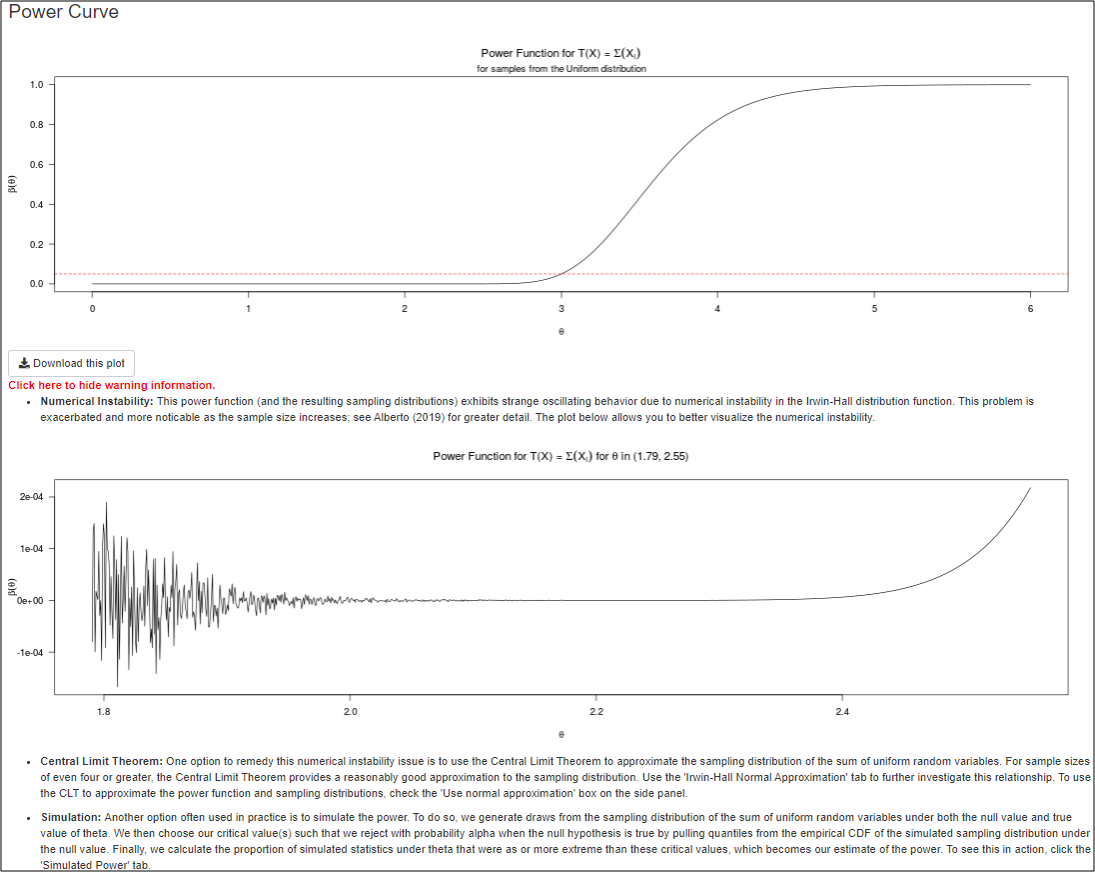
\includegraphics[width=\textwidth]{irwinerror.png}
	\caption{Irwin-hall error}
\end{figure}

\subsubsection{Exploring normal approximation}

The first option this web application offers students to resolve the numerical instability issue is to use the Central Limit Theorem to approximate the sampling distribution of the sum of uniform random variables and therefore the power function. To implement this solution, students need only click the ``Use normal approximation" check box on the side panel, which is only available for this combination of population distribution and statistic. Upon doing so, the power plot and sampling distributions are replaced by those based on a normal approximation (\hl{figure 11}).

\begin{figure}[H]
	\centering
	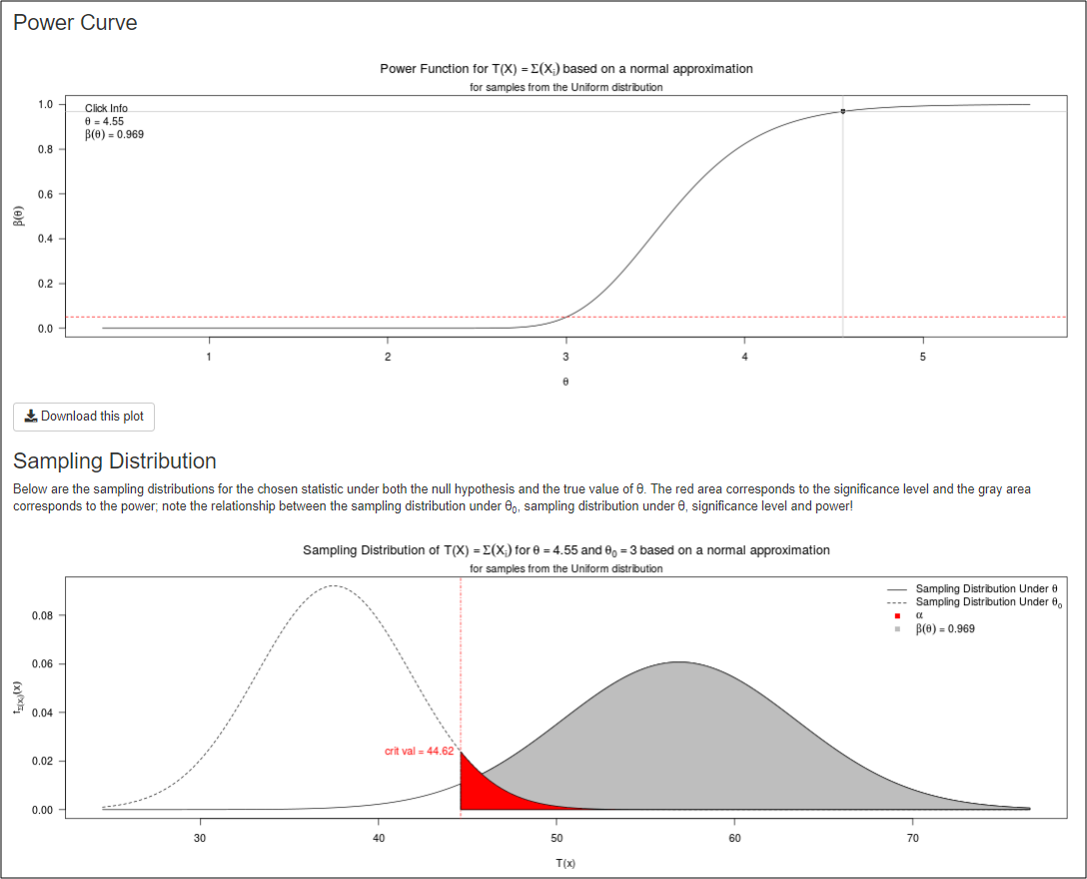
\includegraphics[width=\textwidth]{normapprox1.png}
	\caption{Normal approximation}
\end{figure}

This exploration is valuable for students as it gives them an opportunity to use previously discussed tools to resolve a problem, as a practicing statistician would. This web application also gives students the option to evaluate how well the Central Limit Theorem approximates the sampling distribution of the sum of uniform random variables through the ``Irwin-Hall Normal Approximation" tab. In this tab, students may simulate many samples of a desired size from a uniform($0, \theta$) distribution by specifying the number of simulated samples, sample size, and value of $\theta$ in the sidebar. Students are then able to visualize an approximation of the density function of the sampling distribution with a histogram and view the empirical distribution function. Finally, students may overlay the distribution function of the appropriate normal distribution obtained through the Central Limit Theorem on that empirical distribution function to assess the quality of the approximation (\hl{figure 12}). 

This tab is beneficial for students as it allows them to assess the quality of the approximation used to produce the power function for this test, which is an important part of using the Central Limit Theorem in practice. It also demonstrates how flexible of a tool simulation can be when resolving difficult problems in statistics, which is further explored below. 

\begin{figure}[H]
	\centering
	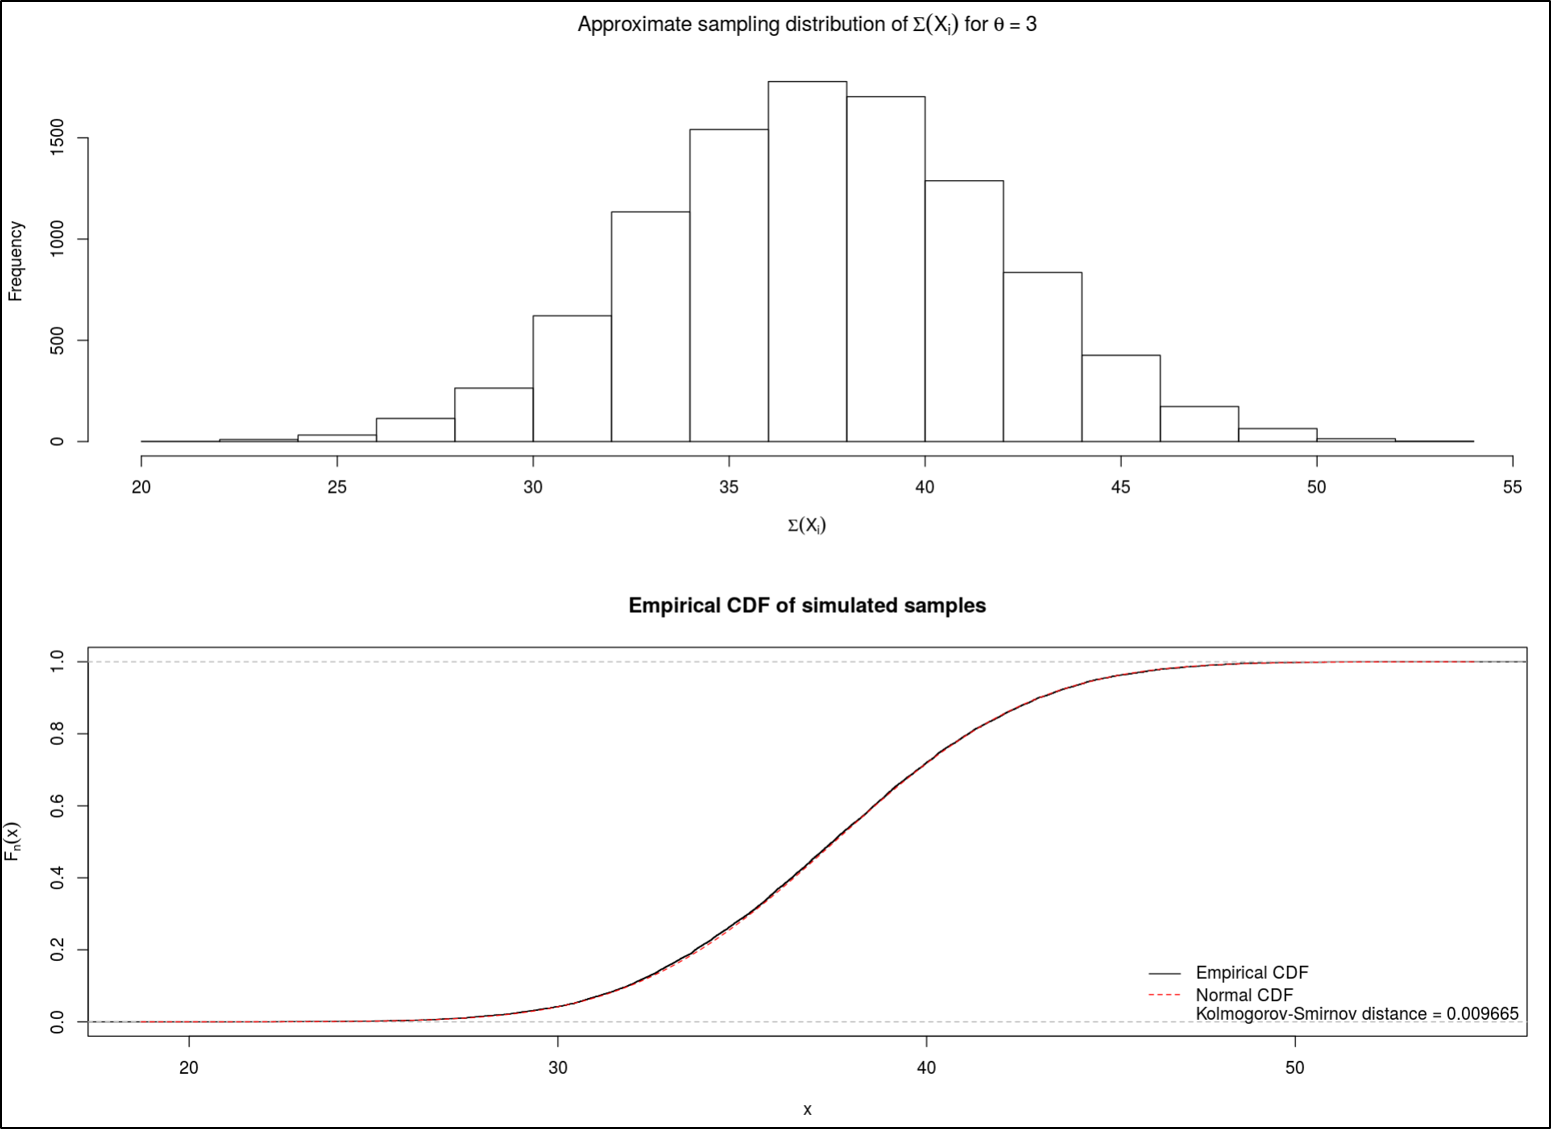
\includegraphics[width=\textwidth]{normapprox2.png}
	\caption{Normal approximation 2}
\end{figure}

\subsubsection{Exploring simulation}

The other option this web application offers students to resolve the numerical instability issue is to use simulation to approximate the sampling distribution of the sum of uniform random variables (and therefore the power function) through the ``Simulated Power" tab. This tab offers a sidebar with options to specify the number of simulated samples, sample size, null value, significance level ($\alpha$), alternative hypothesis, and value of $\theta$. Once specified, students may click the ``Simulate power!" button to produce both the simulated power function and simulated sampling distributions under both the null value and specified value of $\theta$ (\hl{figure 13}).

To create the simulated power function, this web application first  creates a fine sequence of $\theta$ values along the x-axis. Then for each value of $\theta$, this web application simulates the specified number of simulated samples of the specified size (through the sidebar panel) from a uniform($0, \theta$) distribution and calculates the sum of each of those samples (hereafter called the alternative sums); this process is repeated for the specified null value (hereafter called the null sums). Next, the critical value(s) is determined by calculating the the $\alpha^{th}$ percentile of the null sums for a less than alternative, the $(1 - \alpha)^{th}$ percentile of the null sums for a greater than alternative, or the $(\alpha/2)^{th}$ and $(1 - \alpha/2)^{th}$ percentiles of the null sums for a not equal to alternative. Finally, the simulated power is determined by calculating the proportion of alternative sums that is less than or equal to the critical value for a less than alternative, greater than or equal to the critical value for a greater than alternative, or by summing the proportion of alternative sums that is less than or equal to the lower critical value and greater than or equal to the upper critical value for a not equal to alternative hypothesis. The simulated power at each value of $\theta$ is then plotted against $\theta$ to produce the simulated power function. 

\begin{figure}[H]
	\centering
	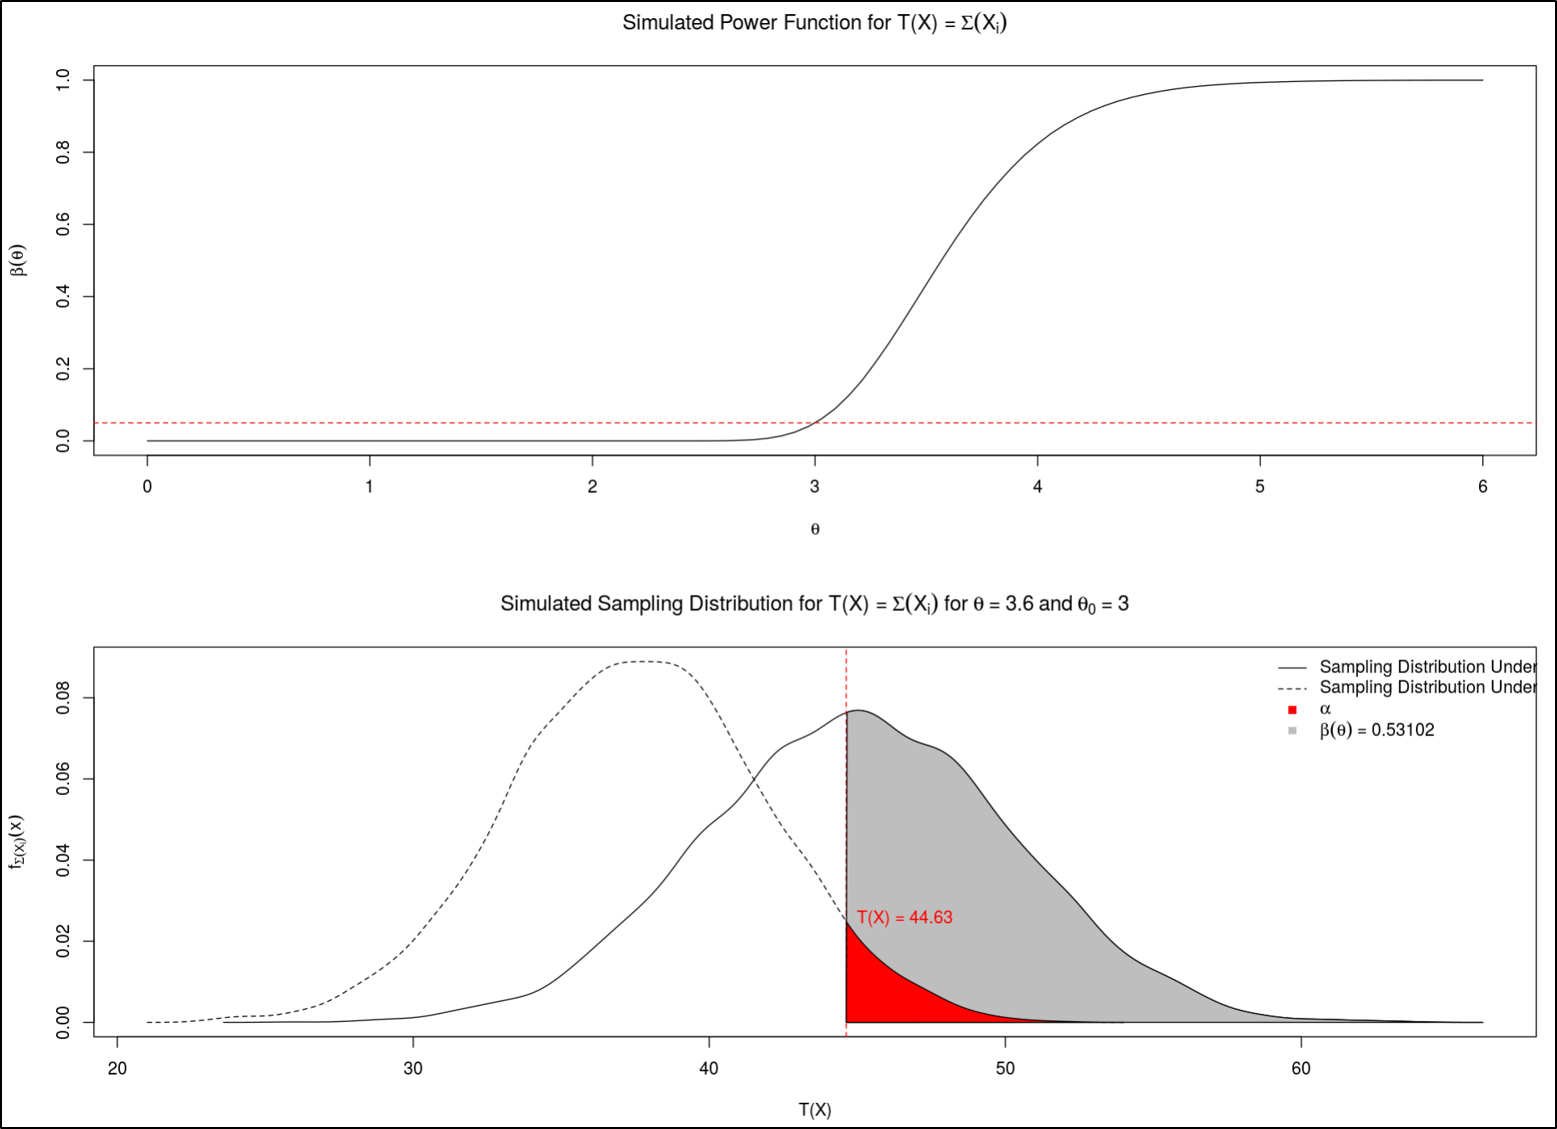
\includegraphics[width=\textwidth]{sim.png}
	\caption{Simulated power}
\end{figure}
 
The simulated sampling distribution plot is created by repeating this process for only the specified (on the sidebar) value of $\theta$, and plotting the density of the resulting null and alternative sums. The shading is done by first determining the appropriate critical values as described above, then shading under each density in the appropriate direction as determined by the alternative hypothesis. The value of this process is two-fold for students. First, they are able to understand through application how powerful of a tool simulation can be for resolving complicated problems in statistics. In many cases, practicing statisticians prefer simulation to analytical methods for power analyses for its ease of implementation and flexibility; this web application gives students the opportunity to witness this firsthand. Second, students develop a deeper conceptual understanding of the relationship between sampling distributions and power by considering how to simulate a power curve. Doing so requires stepping through the process described above, which cements the understanding developed in the previous two sections. 

\section{APPLICATION IMPLEMENTATION}

We were able to implement this web application in the classroom with a guided activity on three separate occasions: with both an undergraduate and graduate level class in the spring on 2018 and with a graduate level class in the spring of 2019. After each of the 2018 and 2019 implementations, the application was revised based on feedback provided by the students leading to a total of three versions of the application, the third of which being described in section 3 and yet to be implemented in the classroom. The first version (implemented in 2018) featured only the exponential population distribution, the sum of random variables and sample minimum as available statistics, less than and greater than as alternative hypotheses, and did not include any additional tabs. The second version of the application (implemented in 2019) added the normal and uniform population distributions, the sample maximum as a possible statistic, included not equal to as an alternative hypothesis, and did not include any additional tabs. At the time of its implementation, the sampling distribution was not available for the sum of random variables from the uniform distribution. Finally, the third version (described in section 3 and yet to be implemented) of the application added the additional tabs described in section 3 as well as the ability to use normal approximation or simulation for the power function for the sum of random variables from the uniform distribution. In the following sections, we describe background information about the classes in which this application was implemented, then describe the guided activity, and conclude with summaries of student reflections about the application. 

\subsection{Background context}

This application was used in both an undergraduate and graduate level course, both of which are part of a two semester sequence in mathematical statistics. The first semester of both courses focuses on building the foundation of probability theory, varying the level of complexity between the undergraduate and graduate level courses. Both courses begin with combinatorics and the axioms of probability, then move towards exploring random variables including transformations and expectations. Following this exploration, students investigate many different named probability distributions, including both discrete and continuous random variables. The penultimate topic in each course is that of multiple random variables, with the graduate level course going into considerably greater detail. Finally, both courses conclude with a discussion of the properties of random samples, focusing on sampling distributions and how they arise. 

In the second semester, when this web application was implemented, the courses diverge. In the undergraduate course, the beginning of the semester focuses largely on sampling from the normal distribution, the Central Limit Theorem, and order statistics. Following these topics, students are introduced to point estimates and spend about a third of the semester investigating method of moments estimators, maximum likelihood estimators, and how to evaluate those estimators based on the concepts of sufficiency and completeness. In this part of the course, students learn to show sufficiency and completeness largely through the exponential family. Once those topics have been discussed, students spend a few weeks exploring uniform, minimum variance, unbiased estimators (UMVUEs) and how to obtain them through various theorems relying largely on the exponential family of distributions. Upon conclusion of this thorough investigation of point estimates, students spend the final five or six weeks of the semester considering hypothesis testing, power, and confidence intervals, focusing largely on likelihood ratio based techniques for hypothesis tests and confidence intervals.

The graduate level course follows a similar outline to the undergraduate course, but goes into greater detail on most topics. For example, when discussing the Central Limit Theorem and sampling distributions, the graduate level course spends time discussing types of convergence and the delta method. When discussing maximum likelihood estimators and methods of evaluating estimators, there is greater emphasis on the asymptotic properties of maximum likelihood estimators, and students learn to prove sufficiency and completeness by the definition, in addition to useful theorems. When exploring UMVUEs, the graduate level students go into far more detail, learning how to directly find the Cramer-Rao lower bound and use Rao-Blackwell theorem to find a UMVUE. Once these explorations into point estimation are the complete, the graduate level students also investigate hypothesis testing, power, and confidence intervals. 

Both the undergraduate and graduate level courses include students with diverse mathematics and statistics backgrounds, typically including students majoring in various types of engineering, ecology, and physical sciences in addition to those seeking mathematics or statistics degrees. Prerequisites for the undergraduate level course include a course in multivariate calculus, with a course in mathematical proof also recommended. Prerequisites for the graduate level course include completion of the full undergraduate sequence (or a similar undergraduate sequence in mathematical statistics), though exceptions are made at the discretion of the instructor. In all three cases where this application was implemented, students were primed to use it by walking through a derivation of one of the power functions featured on the web application in the preceding class. In the following two classes, students were asked to explore various properties of power using the web application through a guided activity, which is discussed in the next section. 

\subsection{Activity layout}

The same activity (\hl{appendix}) was used across all three implementations, and was built around an example assuming an exponential population distribution. On the first day of each implementation, students were divided into small groups and asked to explore one of the five questions provided in part I of the activity. Students were then asked to summarize their group's exploration on a joint word document and give a short three to five minute presentation on what they discovered at the end of class. The structure of the second day differed between the undergraduate and graduate level implementations. In the undergraduate level course, an exploration of the relationship between the power function and sampling distribution through the web application was lead by the instructor at the beginning of class, after which students openly explored other relationships using the application. In the graduate level implementations, students openly explored the relationship between the power function and sampling distribution for the first half of class and discussed what they discovered for the second half of class. In the 2019 implementation, students also explored additional population distributions (which were newly available in that version of the application) which contributed to the discussion. 

Following all three implementations, students were asked to answer a number of discussion questions (\hl{appendix}). The 2019 cohort were asked an additional set of discussion questions related to the additional distribution and statistic options (\hl{appendix}). These responses were used to guide a discussion at the beginning of class on the third day and clarify any lingering questions; the remainder of that third class was used to derive the power function for one of the examples provided on the web application. In addition to guiding a discussion of lingering questions on the third day of class, the student discussion question responses were used to revise each version of the web application and assess the strengths and opportunities of the web application. In the next section, we discuss the themes common to student responses at each implementation and provide some of our own reflections on this application's implementation. 

\subsection{Student reflections}

There were four types of feedback common to all three implementations. The first type of feedback consisted of statements about how the options on the side panel influenced the power curve. A student in the 2018 undergraduate cohort noted that ``the power function [varied] greatly depending on the test statistic used."  This type of comment was extremely common. For example, a student in the 2018 graduate cohort discovered that ``[as] the sample size increases, the power curve becomes steeper." This type of feedback is extremely valuable, as it suggests that this application helped students understand the relationship between each of the options available on the side panel and the power curve, which is one of the learning objectives discussed in section 1. 

The second type of feedback that was common to all three implementations concerned how the application allow students to quickly visualize changes in the power curve. Many students noted that the application's ability to render the power curve in real-time as they changed options on the side panel helped cement their understanding of the effect of each of those factors on the power curve. A student in the 2018 undergraduate cohort stated that ``it was really helpful to be able to hold some inputs constant, while varying others and see how the power curve was affected." Another student in that cohort noted that it was helpful to ``change a parameter and immediately watch the distribution/power curve change with the parameter." Many students in the graduate cohorts echoed this sentiment. One student in the 2019 cohort felt that ``being able to adjust the things we control as researchers and seeing the instant feedback" was helpful. Overall, many students felt that being able to immediately visualize change in the power function and sampling distributions as they changed inputs on the side panel was helpful. 

The third type of feedback we saw frequently described how the application helped the students understand the role of the sampling distribution in calculating power as well as how the sampling distributions are used to determine the critical values of a test. 
A student in the 2018 undergraduate cohort observed that ``the sampling distribution of the [sample minimum] hardly changes with increased sample size, so power does not really change for [the sample minimum] with increased sample size which is vice versa of the [sum of random variables] statistic." This comment demonstrates how the web application both helped students understand how the sampling distribution of a statistic is related to the power function and helped students compare power functions between statistics. Another student in that cohort noted that she ``really liked seeing the relationship between the null and observed sampling distributions... It really solidified the ideas behind power and critical values." This comment exhibits how the visuals provided by this web application help students understand different aspects of deriving a power function, such as determining the critical values. This understanding was mirrored in the graduate cohort. A student in the 2019 cohort described how she used the application to explore the relationship between sampling distributions and power in the following way:

\begin{quote}
	One aspect I found very helpful was being able to select various values of [theta] and seeing how this changed the sampling distribution. Not only did this connect power to the area under the distribution depending on [the significance level] and [theta] but it also allowed us to make connections between power and variance [of the test statistic]. 
\end{quote}

This type of feedback was encouraging to see, as it suggested that this web application helped students better understand the relationship between the sampling distribution and the power curve, which is the second learning objective provided in section 1. 

The final type of feedback students frequently provided consisted of discussions of interesting relationships the students noticed between the power function and previously discussed concepts. For example, students across all three cohorts noticed that power functions based on sufficient statistics tended to provide higher power across the alternative space than those based on other statistics. For example, two students in the 2018 undergraduate cohort noted that ``it is better to use a sufficient statistic to obtain higher power," and that ``when a sufficient statistic is used the power is higher in the alternative space." We again saw similar discussions in the graduate cohorts. One student in the 2018 cohort provided the following reflection:

\begin{quote}
	I find the relationship between complete, sufficient statistics and power intriguing. Are there ways to prove that maximum power is realized when using a complete, sufficient statistic? Is this always the case? For all alpha? In general, what is the relationship between complete, sufficient statistics, uniform minimum variance unbiased estimators, and power?
\end{quote}

The value in these student reflections is two-fold. It both suggests that students are using this application to think critically about power and its relationship to previously discussed concepts and lays the foundation for comparing test functions, which is the topic that follows power. In addition to sufficiency, some students sought to explore other relationships. One student described his exploration in the following way:

\begin{quote}
	I also found exploring the 'extreme' cases to be interesting. For example, what happens when our alternative value of $\theta$ is less than $\theta_0$, but we have a greater than alternative hypothesis? Interestingly, we still have power greater than 0 due to random chance.
\end{quote}

In this reflection, the student used the web application to understand why there is a positive probability of rejecting the null hypothesis over the null parameter space. This kind of feedback is indicative of the kind of insight students may gain by using this web application to explore their curiosities.

In addition to the type of feedback discussed above, students were asked to provide suggestions for improvements to the web application. In the 2018 implementation, students in both the undergraduate and graduate level courses noted that it would be useful to consider more population distributions, additional statistics, and to explore a not equal to alternative hypothesis. These suggestions lead to the development of the second version of the web application, which added the normal and uniform distributions, sample maximum as a test statistic, and not equal to alternative hypothesis. These changes were associated with a new type of common feedback in the 2019 implementation, which concerned distribution specific observations. For example, one student noted that ``changing theta doesn't affect the variation of the normal distribution whereas it does affect the exponential distribution." This feedback was exciting to see, as it suggested that the additional options available in the second version of the web application helped students gain additional insight into what factors affect the power function. Another student from that cohort summarized this effect: "[The additional options] helped me see that power curves don't always look similar and that changing distribution will drastically change the form of the [power] curve." Students were again asked for suggestions to improve the web application in the 2019 implementation. Some students requested that the derivations for these power function be made available, which lead to the addition of the derivations tab on the current version of the application. 

\section{FUTURE WORK AND CONCLUSIONS}



\newpage
\bibliography{references}

\newpage

\textit{Varying the population distribution}

\begin{quote}
	\textit{Choose the sample maximum as the test statistic and greater than as the alternative hypothesis. Holding all other values constant, what happens to the power curve as the population distribution changes between exponential, normal, and uniform? Why?}
\end{quote}

\begin{quote}
	\textit{Which power function is closest to an ideal power curve? Why?}
\end{quote}

\textit{Varying the test statistic}

\begin{quote}
	\textit{Choose the uniform distribution as the population distribution and not equal to as the alternative hypothesis. Holding all other values constant, compare the power functions for each of the available test statistics. Which statistic provides the highest power across the alternative space?}
\end{quote}

\begin{quote}
	\textit{Switch the population distribution to the normal distribution and repeat the previous exercise. Explain why your answer to each of these questions differs.}
\end{quote}

\textit{Varying the alternative hypothesis}

\begin{quote}
	\textit{Choose the exponential distribution as the population distribution and sum of the X's as the statistic. Holding all other values constant, what happens to the power curve as the alternative hypothesis changes between greater than, less than, and not equal to? Why?}
\end{quote}

\begin{quote}
	\textit{Why is the power function not symmetric about the null value?}
\end{quote}

\begin{quote}
	\textit{Choose the uniform distribution as the population distribution, sample maximum as the statistic, not equal to as the alternative hypothesis, and set the sample size to one. Is this test unbiased? Why or why not?}
\end{quote}

\textit{Varying the significance level}

\begin{quote}
	\textit{Choose any combination of population distribution and statistic. Holding all other values constant, what happens to the power function as the significance level increases? Why?}
\end{quote}

\begin{quote}
	\textit{Explain how the significance level affects the power curve in terms of the type I error rate. What trade-offs are made in terms of the probability of making a type II error when increasing the significance level? (Hint: recall that the power of a test is equal to one minus the probability of a type II error)}
\end{quote}

\textit{Varying the null value}

\begin{quote}
	\textit{Choose any combination of population distribution and statistic. Holding all other values constant, what happens to the power function as you change the null value? Why does this happen?}
\end{quote}

\begin{quote}
	\textit{Explain the relationship between the power function, null value, and significance level.}
\end{quote}

\textit{Varying n}

\begin{quote}
	\textit{Choose the normal distribution as the population distribution, sum of the X's as the test statistic, and not equal to as the alternative hypothesis. Holding all other values constant, what happens to the power function as the sample size increases? Why?}
\end{quote}

\begin{quote}
	\textit{Change the statistic to the sample minimum. What happens to the power function as the sample size increases?}
\end{quote}

\begin{quote}
	\textit{Why do you think the effect of the sample size on the power curve is lesser for the sample minimum than for the sum of the X's?}
\end{quote}

\textit{Sampling distributions}

\begin{quote}
	\textit{Choose the exponential distribution as the population distribution, sum of the X's as the test statistic, greater than as the alternative hypothesis, a sample size of 25, and set the null value and theta to be three and four respectively. Describe where each of the distributions plotted under the Sampling Distribution heading is centered and what each distribution represents. Hint: recall that the distribution of the sum of $n$ exponential($\theta$) random variables is gamma($n, \theta$).}
\end{quote}

\begin{quote}
	\textit{Describe what the red and grey shaded areas represent. How is the red area used to determine the grey area?}
\end{quote}

\begin{quote}
	\textit{Which of the factors on the sidebar panel that affect each of these sampling distributions are controlled by the researcher and which are unknown? Based on your answer, how would you recommend a researcher increases the power of their hypothesis test?}
\end{quote}


\end{document}